This section reports the experimental validation of our model.
We begin by 
testing the model on real data (section \ref{res:real}), showing that
by joint modeling visual and motor information it is possible to
achieve a significant boost in recognition, compared to using visual
information only. 
We proceed evaluating the quality of the reconstructed archetypal grasp via regression
(section \ref{res:regression}).
We then show that, whenever the motor information
is not perceived by the agent, it is still possible to get a better performance
by using our VMM to generate an archetypal grasp as input for the classifier
(section \ref{res:reconstruct}).



%The visual / motor grasping data used to build the VMM is contained in
%the CONTACT Visuo-Motor Grasping dataBase (VMGdB). The VMGdB is obtained
%by having $20$ subjects repeatedly grasp $7$ objects in $5$ different ways;
%meanwhile, two Watec \emph{WAT-202D} colour cameras and a $22$-sensors
%Immersion \emph{CyberGlove} \cite{cyberglove} right-hand sided dataglove
%were used to obtain a fair visual / motor representation of the grasping acts.
%Absoute timestamps are used to synchronise the video and numerical streams.
%In this setting we only used one of the cameras, focussed on the object and
%lateral to the subject; the dataglove provides $22$ $8$-bit numbers
%linearly related to the angles of the subject's hand joints.

%The VMGdB purposedly enforces no control over the illumination of the set-up,
%nor any guarantee on the colours of objects or of the background; moreover,
%each object has been grasped in several different ways, and the same grasp
%has been used for several different objects. This makes the VMGdB
%a realistic representation of the act of grasping an object.


\subsection{Results with real motor data}
\label{res:real}

The first set of experiments was conducted on real data, namely motor data
registered by the users when grasping the objects, and the corresponding images.
Our goal here was to show the advantage in recognition achieved by modelling the object
on both modalities, and at the same time compare the three possible joint
modelling strategies presented in section \ref{sec::classifier}, to chose the best one.

Experiments were performed considering the whole set
of 5200 data and choosing randomly 130 samples for
training and 2600 samples for testing. The random extraction was repeated
defining 10 different splits and the classification was executed using SVM,
one-vs-all multiclass extension. We used the Gaussian Kernel for the
visual and motor modalities, both when considered separately and in the
integration approach (two Gaussian Kernels combined in MCK). The best
learning parameters were selected through cross validation.

% \begin{table*}[tbp]
% \centering \footnotesize
% \begin{tabular}{c|@{}c@{}|@{}c@{}|@{}c@{}|@{}c@{}|@{}c@{}|@{}c@{}|@{}c@{}|@{}c@{}|@{}c@{}|@{}c@{}|@{}c@{}|@{}c@{}|@{}c@{}|@{}c@{}|@{}c@{}|@{}c@{}|@{}c@{}|@{}c@{}|@{}c@{}|@{}c@{}|@{}c@{}|@{}c@{}|@{}c@{}|}
%   \cline{2-8} \cline{10-16} \cline{18-24}
%   % after \\: \hline or \cline{col1-col2} \cline{col3-col4} ...
% \multirow{7}{*}{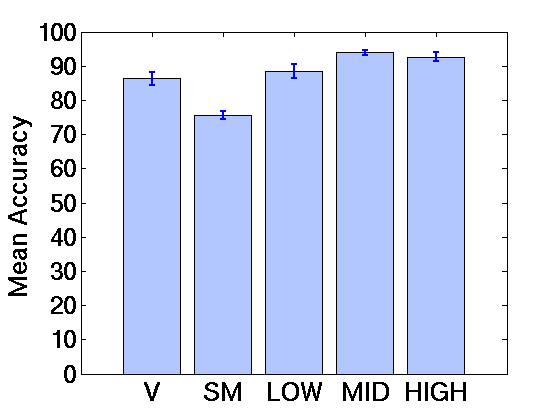
\includegraphics[width=0.18\textwidth]{images/real}}& 88.6&	0.9&	1.4&	1.0&	7.2&	0.4&	0.5&&	77.2&	0.3&	0.3&	0.7&	0.4&	19.9&	1.2&&	96.5&	0.1&	0.0&	0.9&	1.2&	1.2&	0.2\\
%   \cline{2-8} \cline{10-16} \cline{18-24}
% &0.1&	80.9&	0.1&	0.3&	16.5&	0.0&	2.2&&	1.1&	58.9&	25.3&	1.2&	2.0&	9.5&	2.1&&	0.0&	91.8&	2.5&	1.1&	2.8&	1.4&	0.5\\
%   \cline{2-8} \cline{10-16} \cline{18-24}
% &3.4&	0.2&	88.3&	0.3&	4.3&	2.8&	0.6&&	0.5&	5.7&	79.0&	0.5&	0.9&	8.6&	4.9&&	0.1&	1.8&	94.4&	0.1&	0.3&	2.5&	0.8\\
%   \cline{2-8} \cline{10-16} \cline{18-24}
% &0.0&	0.0&	0.4&	75.1&	24.5&	0.0&	0.0&&	2.6&	0.6&	0.2&	96.6&	0.0&	0.2&	0.0&&	0.0&	0.0&	0.0&	100.0&	0.0&	0.0&	0.0\\
%   \cline{2-8} \cline{10-16} \cline{18-24}
% &0.7&	1.6&	1.9&	1.3&	90.4&	1.6&	2.7&&	0.0&	0.8&	0.5&	0.0&	77.7&	0.3&	20.9&&	0.0&	0.1&	0.0&	0.1&	88.4&	0.0&	11.4\\
%   \cline{2-8} \cline{10-16} \cline{18-24}
% &0.0&	0.0&	0.0&	0.1&	1.8&	98.1&	0.0&&	13.0&	1.7&	6.8&	0.3&	0.9&	70.7&	6.7&&	0.7&	0.2&	0.2&	0.1&	0.6&	98.0&	0.2\\
%   \cline{2-8} \cline{10-16} \cline{18-24}
% &2.2&	2.4&	3.1&	1.2&	7.1&	0.9&	83.2&&	0.3&	4.8&	1.2&	0.8&	17.9&	6.3&	68.7&&	0.4&	2.0&	0.2&	0.4&	7.2&	1.4&	88.5\\
%   \cline{2-8} \cline{10-16} \cline{18-24}
% \multicolumn{1}{c}{} &\multicolumn{7}{c}{} &\multicolumn{1}{c}{}& \multicolumn{7}{c}{} &\multicolumn{1}{c}{}& \multicolumn{7}{c}{}\\
% \multicolumn{1}{c}{\normalsize(a)} &\multicolumn{7}{c}{\normalsize(b)} &\multicolumn{1}{c}{}& \multicolumn{7}{c}{\normalsize(c)} &\multicolumn{1}{c}{}& \multicolumn{7}{c}{\normalsize(d)}\\
% \end{tabular}
% \caption{}
% \label{table1}
% \end{table*}

\begin{figure*} \centering
  \begin{tabular}{@{}c@{}@{}c@{}@{}c@{}}
    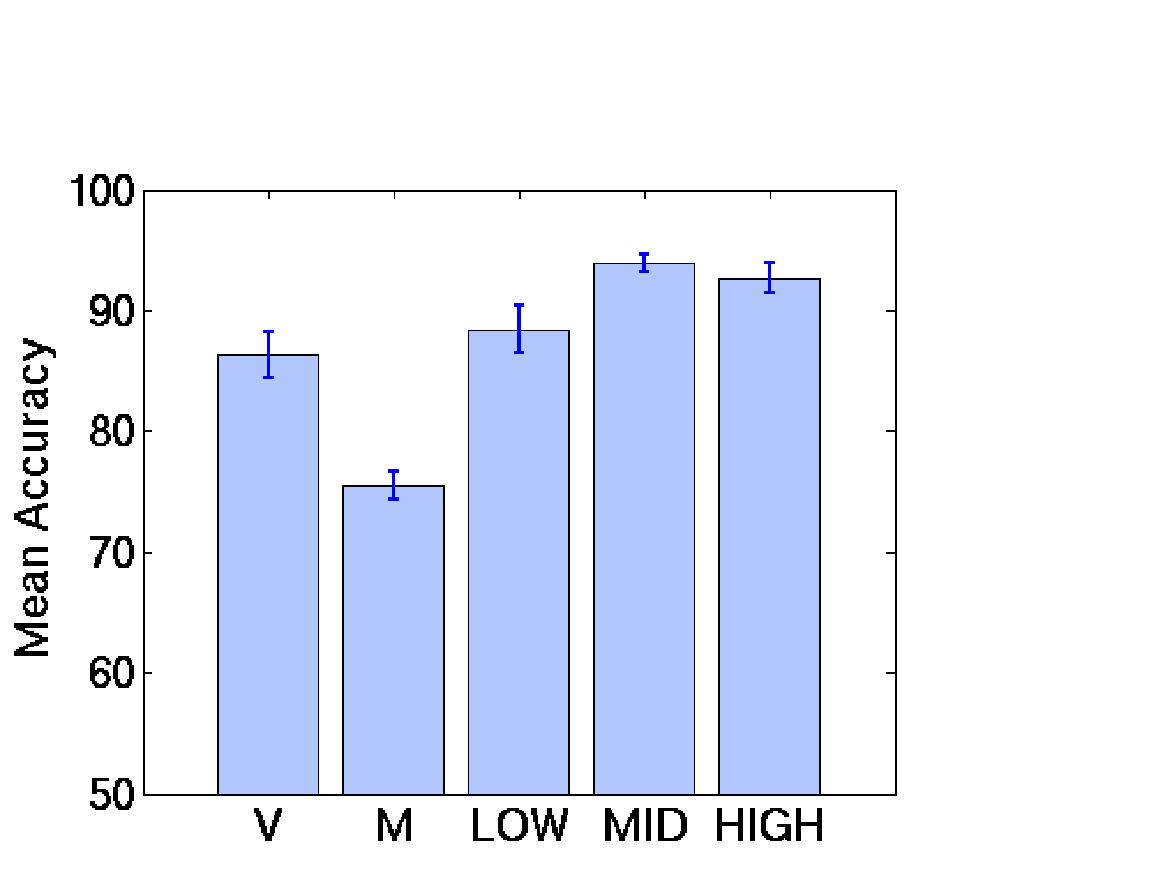
\includegraphics[width=0.25\textwidth]{images/real_.pdf} &
    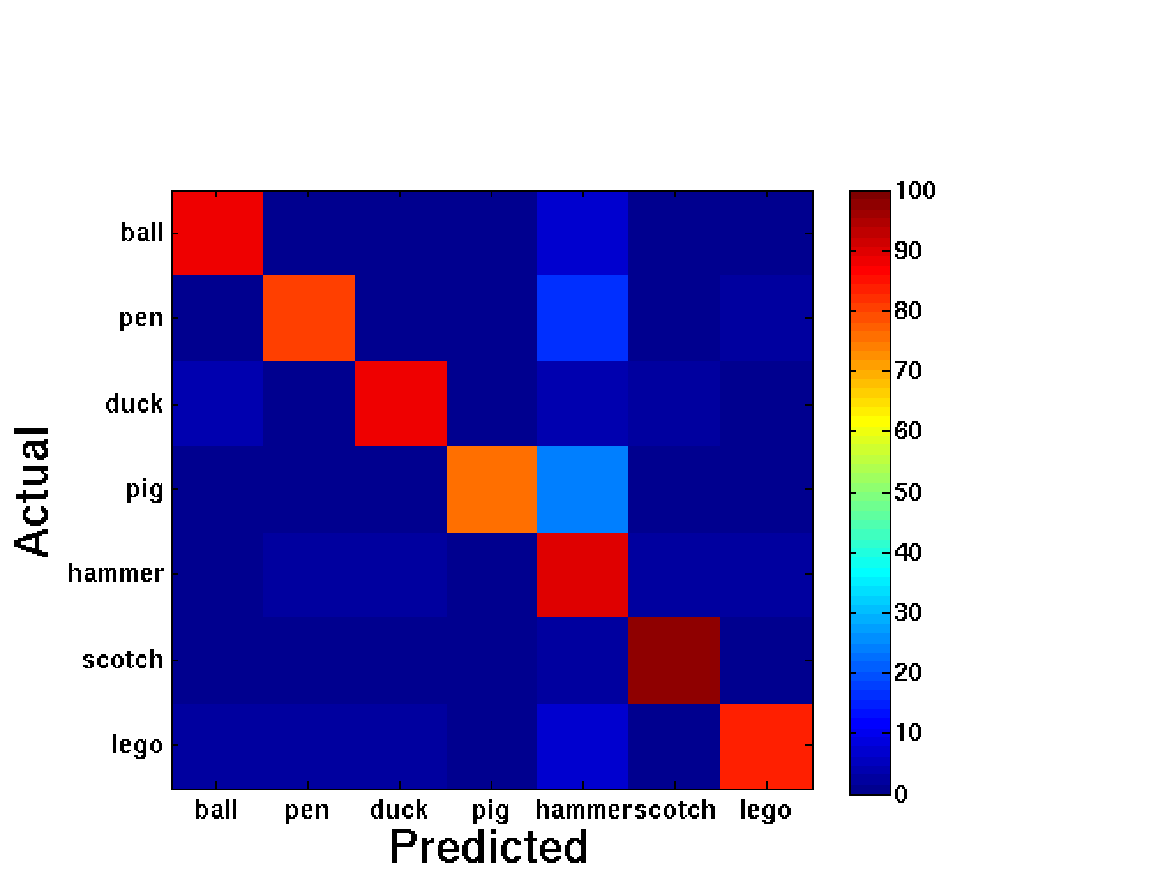
\includegraphics[width=0.25\textwidth]{images/conf_vis.pdf} &
    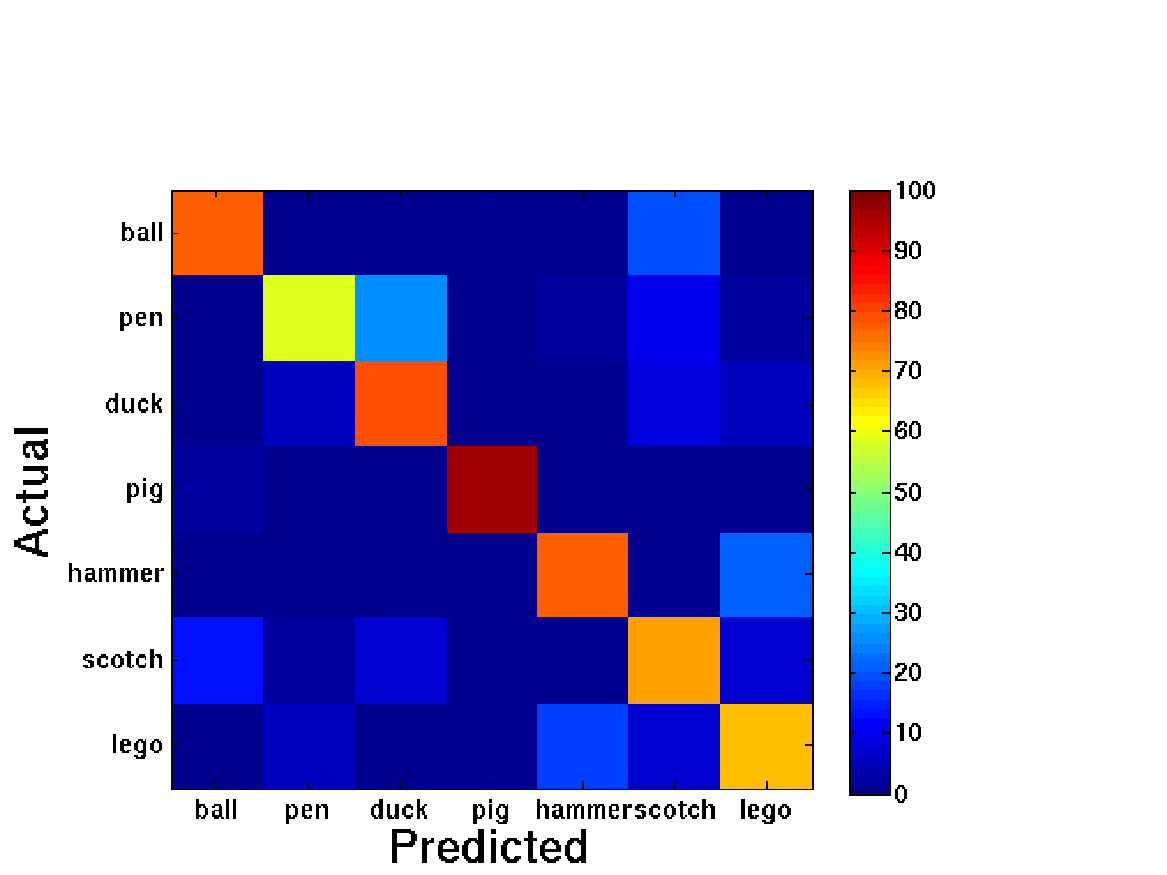
\includegraphics[width=0.25\textwidth]{images/conf_mot.pdf} \\
(a) & (b) & (c)\\
    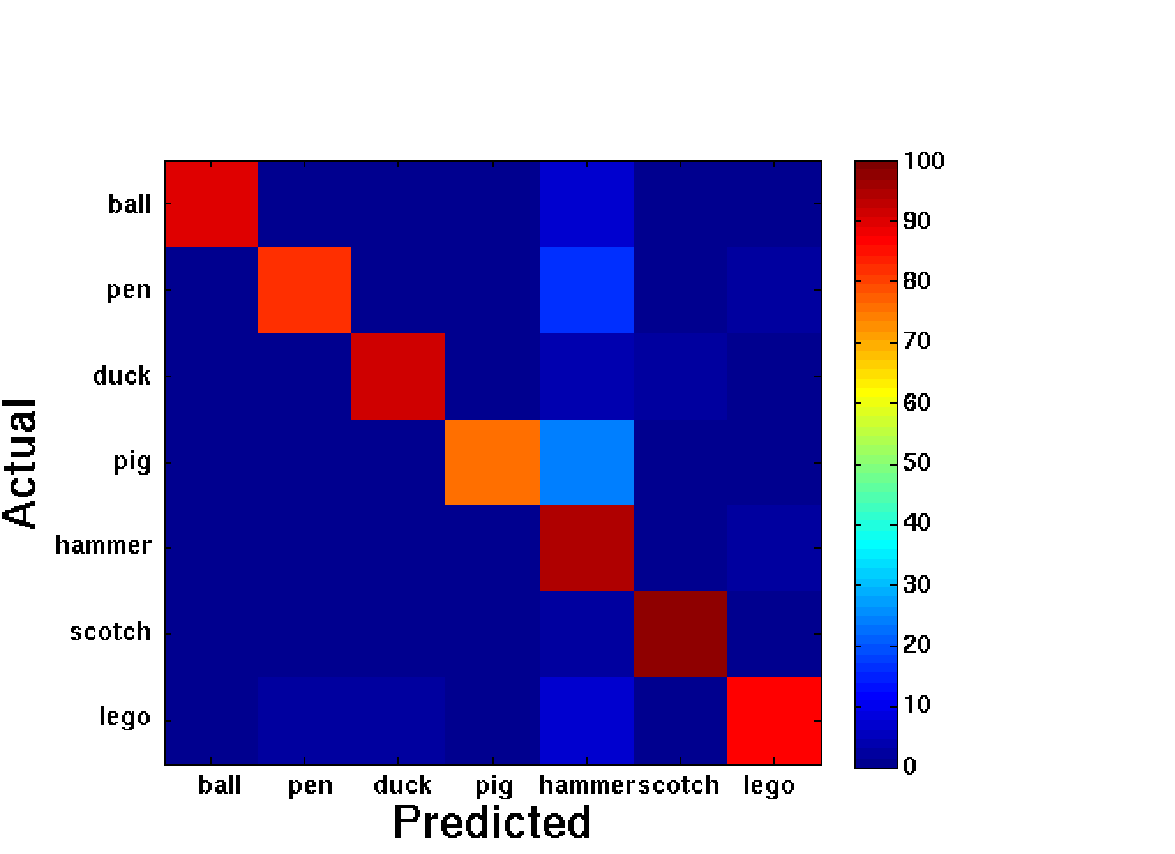
\includegraphics[width=0.25\textwidth]{images/conf_low_real.pdf} &
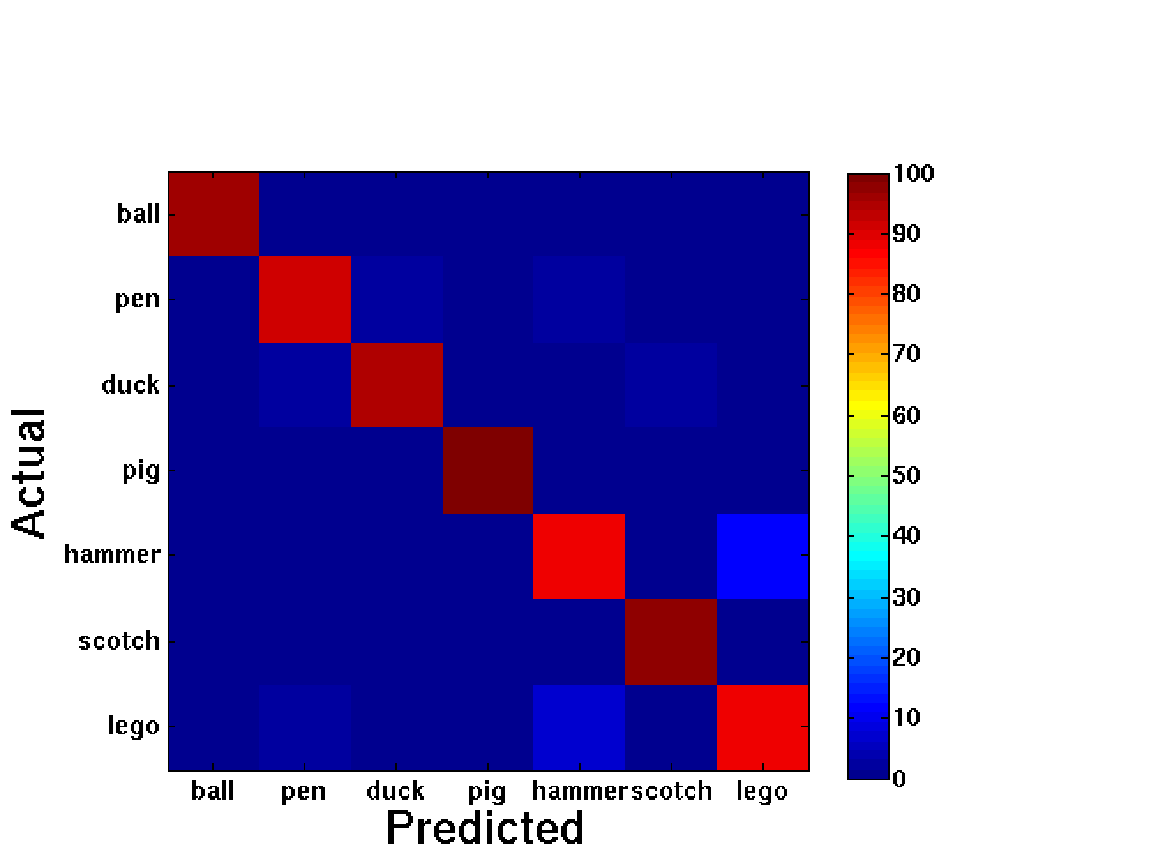
\includegraphics[width=0.25\textwidth]{images/conf_mck_real.pdf} &
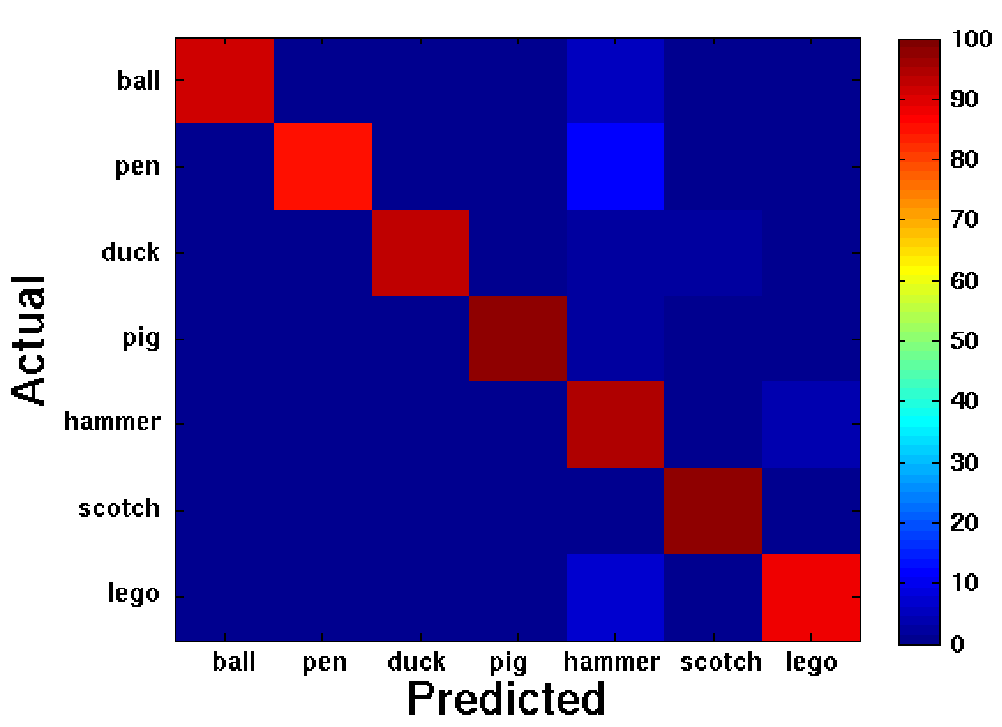
\includegraphics[width=0.25\textwidth]{images/conf_das_real.pdf} \\
    (d) & (e) & (f)\\
  \end{tabular}
  \caption{(a) Classification mean accuracy of the seven objects averaged
    on the ten splits; (b) confusion matrix using visual features; (c) confusion
    matrix using motor features; (d) confusion matrix using the low level
    feature integration; (e) confusion matrix using the mid level
    feature integration; (f) confusion matrix using the high level
    feature integration.}
  \label{fig:real_data}
\end{figure*}

Figure \ref{fig:real_data}-a shows the overall recognition results obtained by using only visual
information (V), only motor information (M), or the two combined together, with the three proposed approaches (LOW, MID, HIGH). We see in general that using the visual information we obtain better average performance ($86.37\%\pm1.91\%$) than using the motor one
($75.53\%\pm1.22\%$), and that their integration is clearly beneficial. The mid-level integration produces the best result ($93.94\%\pm0.77\%$): the gain in accuracy between MCK and only using visual features is $7.57\%$ (difference in accuracy
evaluated per split and then averaged on the 10 splits).
The second best result is obtained by using DAS ($92.65\%\pm 1.22\%$); we see that the difference in performance between DAS and MCK is 
not statistically significant, and therefore both are suitable candidates for the VMC module. 


Figure \ref{fig:real_data}-b, -f 
shows the confusion matrices obtained by the vision only classifier (Figure  \ref{fig:real_data}-b), by the 
motor only classifier (Figure \ref{fig:real_data}-c) and by the 
three integration methods: low-level (Figure \ref{fig:real_data}-d),
MCK  (Figure \ref{fig:real_data}-e)
and DAS (Figure \ref{fig:real_data}-f). 
It is clear that the combination of the two modalities leads to considerable 
advantages in the recognition of each object, for all methods. 
Consider for instance  the objects ``ball'' and ``pig'':  the mean accuracy is
respectively $88.6\%$ and $75.1\%$ using visual features and $77.2\%$ and $96.6\%$ using motor information. 
The ball was grasped in two different ways (with a `tripodal'' and a ``spherical'' grasp)
while the pig was manipulated only with the ``cylindric'' grasp, which was used just for this object.  
Thus, the grasp information is object-specific for the pig.
This led to an impressive increase in performance when using MCK, as we achieved a 100\% classification rate. Using
visuo-motor information is beneficial also for the ball, for which we obtained a multi modal recognition rate of 96.5\%.
Analogous considerations can be done for the two other approaches, and are omitted here for space reasons.

%For the
%``pen'', the ``tripodal'' and the ``spherical'' grasps were registerd while the ``pig'' was manipulated only with the ``cylindric'' grasp, which was used just for this object.  Thus, the grasp information is object-specific for
%the ``pig'' and this led to a good performance when using the motor data in object classification. With MCK we obtain respectively $96.5\%$ and $100.0\%$ for the ``pen'' and the ``pig''. 


From these experiments we can conclude that: (a) using a joint visual and motor object model leads to a very concrete 
advantage in performance during recognition, and (b) the MCK algorithm seems the most suitable for the joint 
modelling of the two modalities.

\subsection{Evaluation of reconstructed data}
\label{res:regression}
We now turn to the evaluation of the archetypal grasps generated by the VMM. We learn a neural network for each object seen during training; this results here in seven specific VMMs. If an object can be grasped in
only one way, the reconstructed motor data correspond to an estimate of this
grasp type. If the possible grasps are more than one, the reconstructed motor data
represent an estimate of the ``average'' grasp for that object.

To evaluate the goodness of the VMM in producing ``archetypal grasps'', we performed the following experiment:
 we divided the whole
dataset in two halves (2600 data each), using one for training and the other for testing. Specifically
we used the samples to:
\begin{enumerate}

  \item [(a)] Train the neural networks and predict the motor feature vectors of the
    testing set, for each
VMM associated to its specific object.	
 %using the correct object label for each. In this way we eliminate the uncertanity
 %   on which neural network should be used and evaluate the reconstructed sensorimotor vectors
 %   classifying them in terms of grasps.

  \item[(b)] Train a ``grasp classifier'' on the real motor information. The testing phase consisted
    in predicting the grasp label of the reconstructed motor vectors obtained from (a).
    We counted as  an error every time the predicted grasp was not one of the possible grasps
    associated with the relative object.

\end{enumerate}

We run the experiment on 10 splits of the whole dataset and we obtained an average error rate of
10.7\%. This is significantly low with respect to a random grasp labelling (error rate of 63\%).
We can conclude that the reconstructed grasp information is coherent with the real one, and therefore we expect 
that the archetypal grasp will turn out to be an informative feature when used for classification. 



%The most frequent case is of course that of an agent seeing an object without grasping it. 
%In that case, we propose an approach which still permits to take advantage from the VMM
%learned during training. More in detail:

%\noindent\textbf{Training}:  we consider a neural network for each object in
%the training phase resulting in 7 specific VMMs. If an object can be grasped in
%only one way, the reconstructed motor data correspond to an estimate of this 
%grasp type. If the possible grasps are more than one, the reconstructed motor data
%represent an estimate of the ``average'' grasp for that object.
%
%\noindent\textbf{Testing}: our system performs three steps:
%\begin{enumerate}
%  \item the VPR is extracted from the visual appearance of the object. Based upon
%    it, the label of the object is predicted;
%  \item this label is used to choose the appropriate VMM;
%  \item the VMM reconstructs the grasp associated with the object and this
%    MPR is then used, alone or joined with the VPR, to recognize the object.
%\end{enumerate}
%
%
%To begin with, it is important to evaluate the goodness of the VMM in producing ``archetipal grasps''.
%This means isolating the VMM performance not considering the object guessing
%in the first step of the recognition strategy in the test phase. To this end we divided the whole 
%dataset in two halves (2600 data each) using one for training and the other for testing. Specifically 
%we used the samples to:
%
%\begin{enumerate}
%
%  \item [(a)] train the neural networks and predict the sensorimotor feature vectors of the 
%    testing set using the correct object label for each. In this way we eliminate the uncertanity 
%    on which neural network should be used and evaluate the reconstructed sensorimotor vectors
%    classifying them in terms of grasps.
%
%  \item[(b)] train a ``grasp classifier'' on the real motor information, the testing phase consisted 
%    in predicting the grasp label of the reconstructed sensorimotor vectors obtained from (a). 
%    We considered an error each time the predicted grasp is not one of the possible grasps 
%    associated with the seen object. 
%
%\end{enumerate}
%
%We run the experiment on 10 splits of the whole dataset and we obtained an average error rate of
%10.7\% which is significativly low respect to a random grasp labelling (error rate of 63\%).
%This tells us that the reconstructed grasp information is coherent with the real one.
%

\subsection{Results with reconstructed data}
\label{res:reconstruct}


The most frequent case is of course that of an agent seeing an object without grasping it. 
In that case, our approach  still permits to take advantage of the VMC, using as 
motor input the archetypal grasp generated by the VMM.
More in detail, the system 
performs three steps (see Figure \ref{fig::reconstructed-schema} for a schematic representation):
\begin{enumerate}
  \item We extract the visual features  from the object's view. Based upon
    it, we generate an hypothesis on %predict 
	the label of the object using only visual data. 
%with a vision-only classifier;
  \item The hypothesis is used to choose the appropriate VMM.
  \item The VMM reconstructs the grasp associated with the object. This
    motor feature is then used, alone or jointly with the visual feature, to recognize the object.
\end{enumerate}
We evaluated this strategy by repeating the experiments described in Section \ref{res:real}, using as input only visual data.
For the implementation of the first step described above, we used the vision only classifier trained on real data
(see Section \ref{res:real}).


\begin{figure}
        \centering
        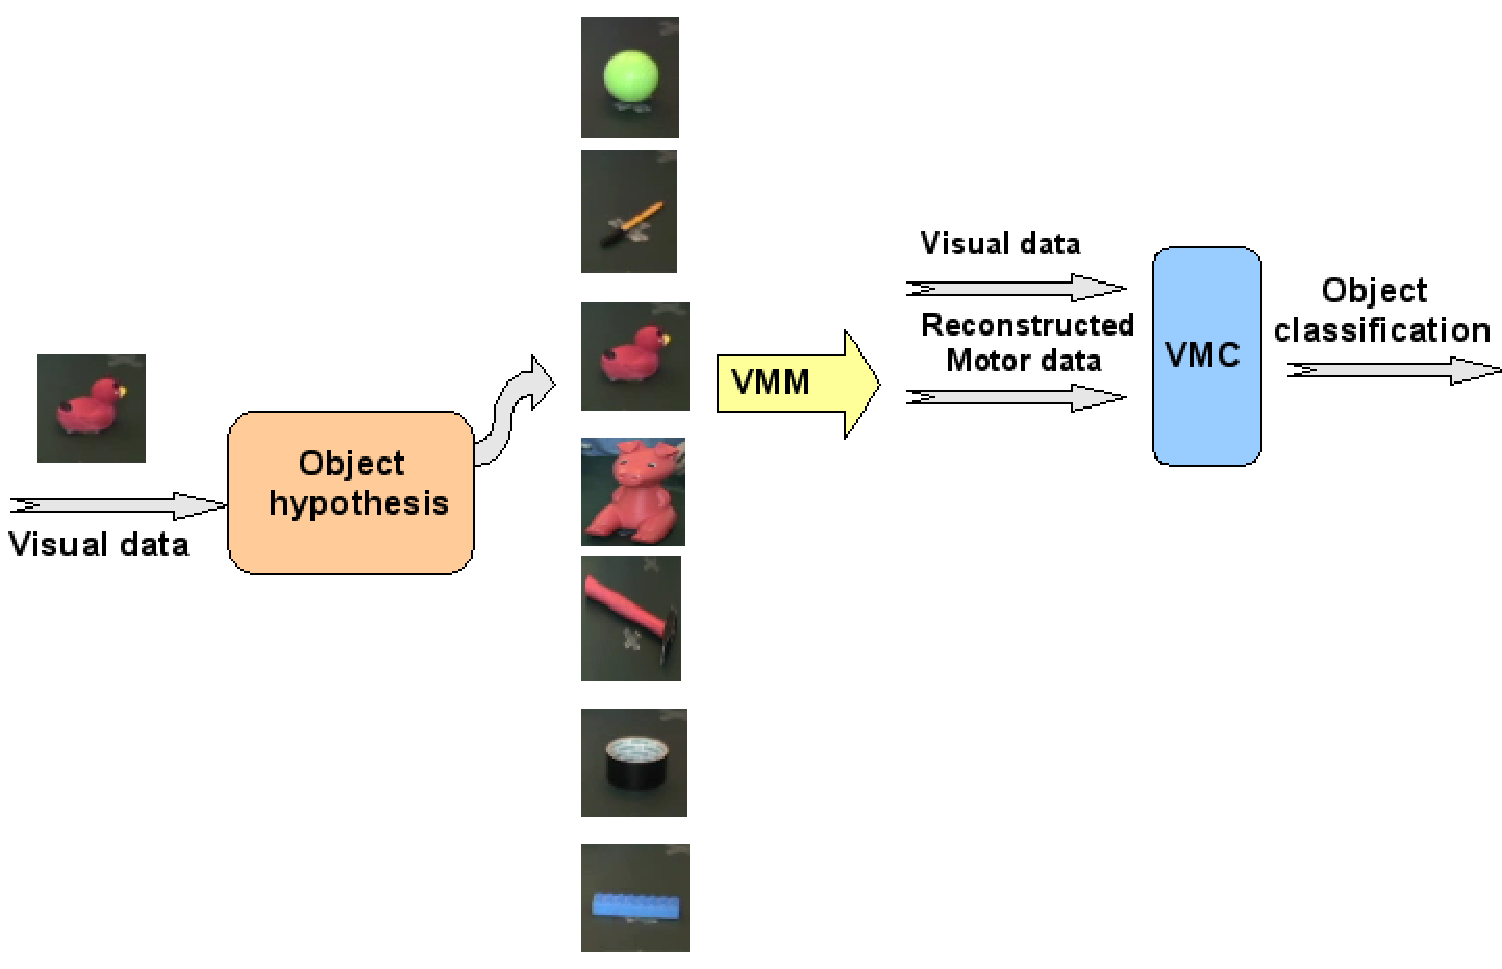
\includegraphics[width=0.5\textwidth]{images/schema_process.pdf}
        \caption{A schematic representation of how the reconstructed motor features are used in the VMC.}
        \label{fig::reconstructed-schema}
\end{figure}



 
%We repeated the classification experiments described in section \ref{res:real}, using as input only visual data. 
%We considered all the three steps defined in section \ref{res:regression}, using for the first one 
%the classifier on visual information (V) obtained from the set of
%experiments on real data.

\begin{figure*} \centering
  \begin{tabular}{@{}c@{}@{}c@{}@{}c@{}}
    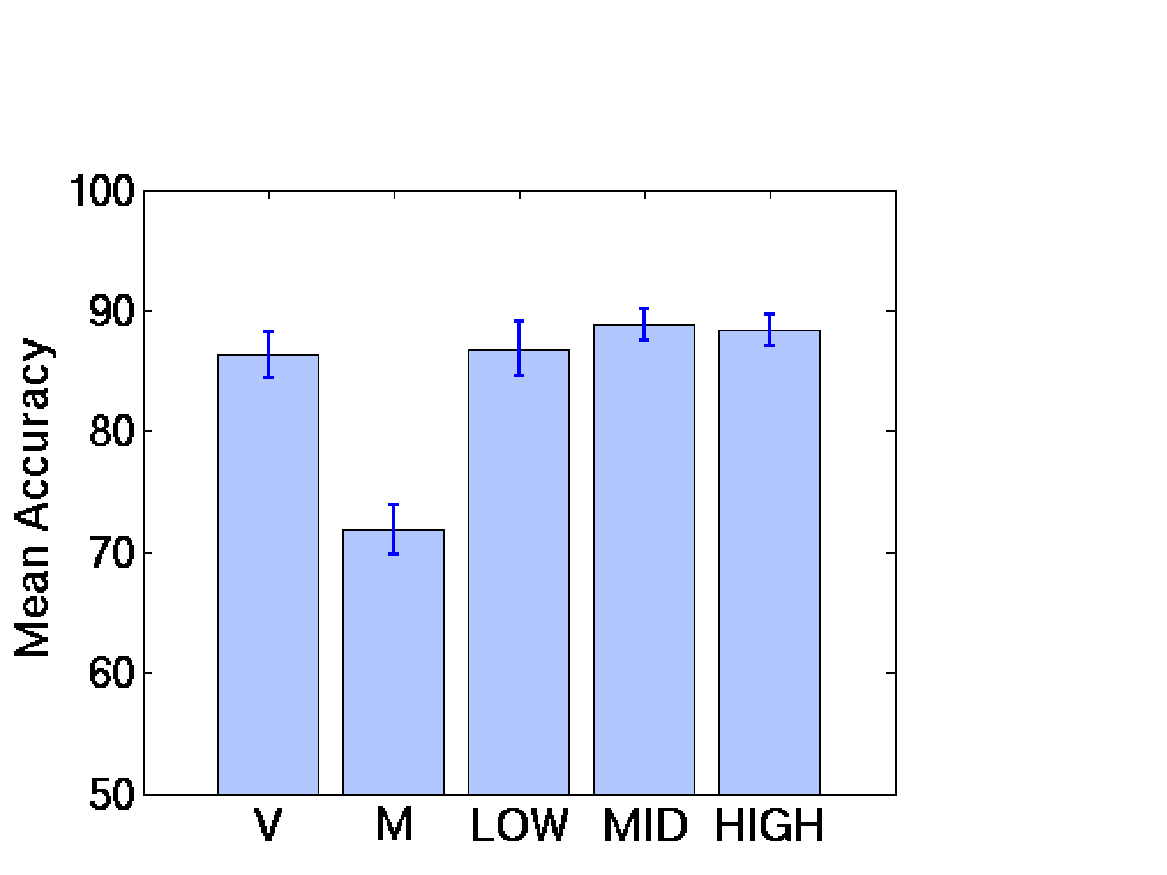
\includegraphics[width=0.25\textwidth]{images/ric_.pdf} &
    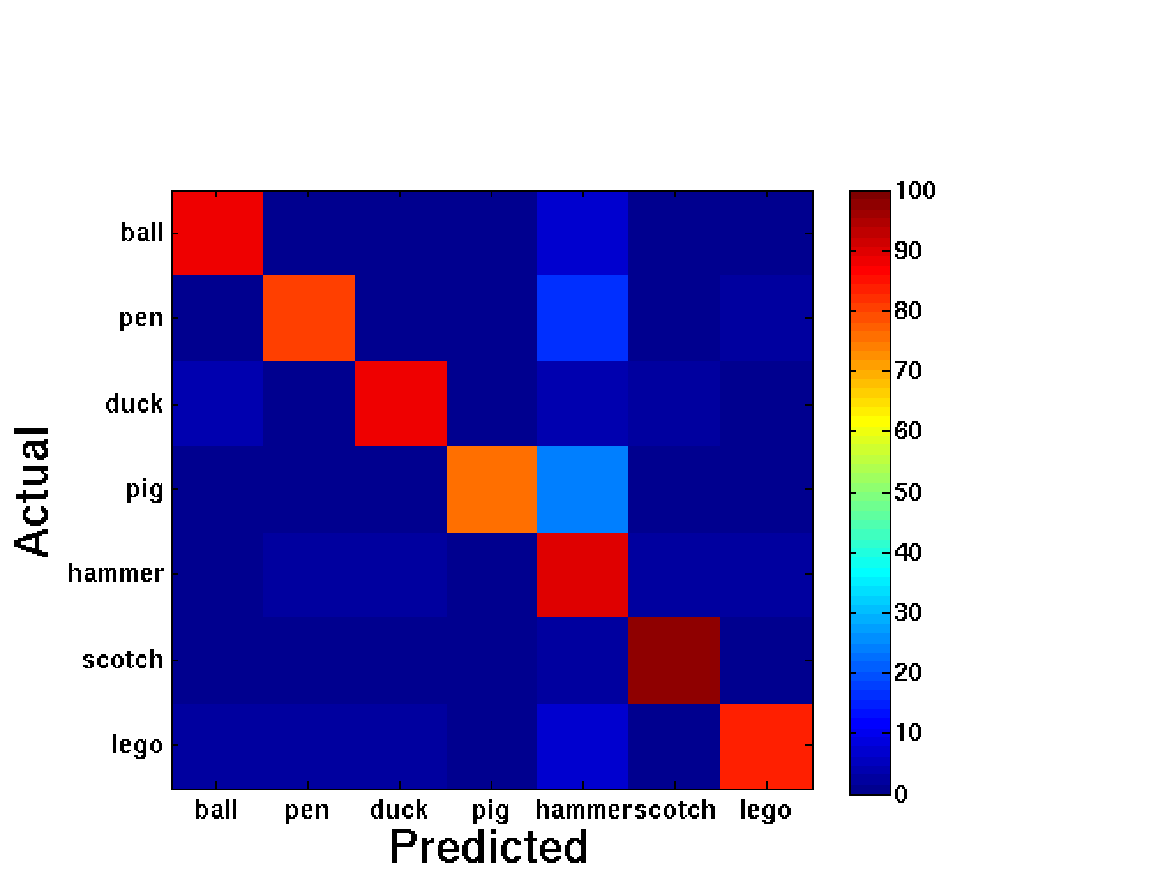
\includegraphics[width=0.25\textwidth]{images/conf_vis.pdf} &
    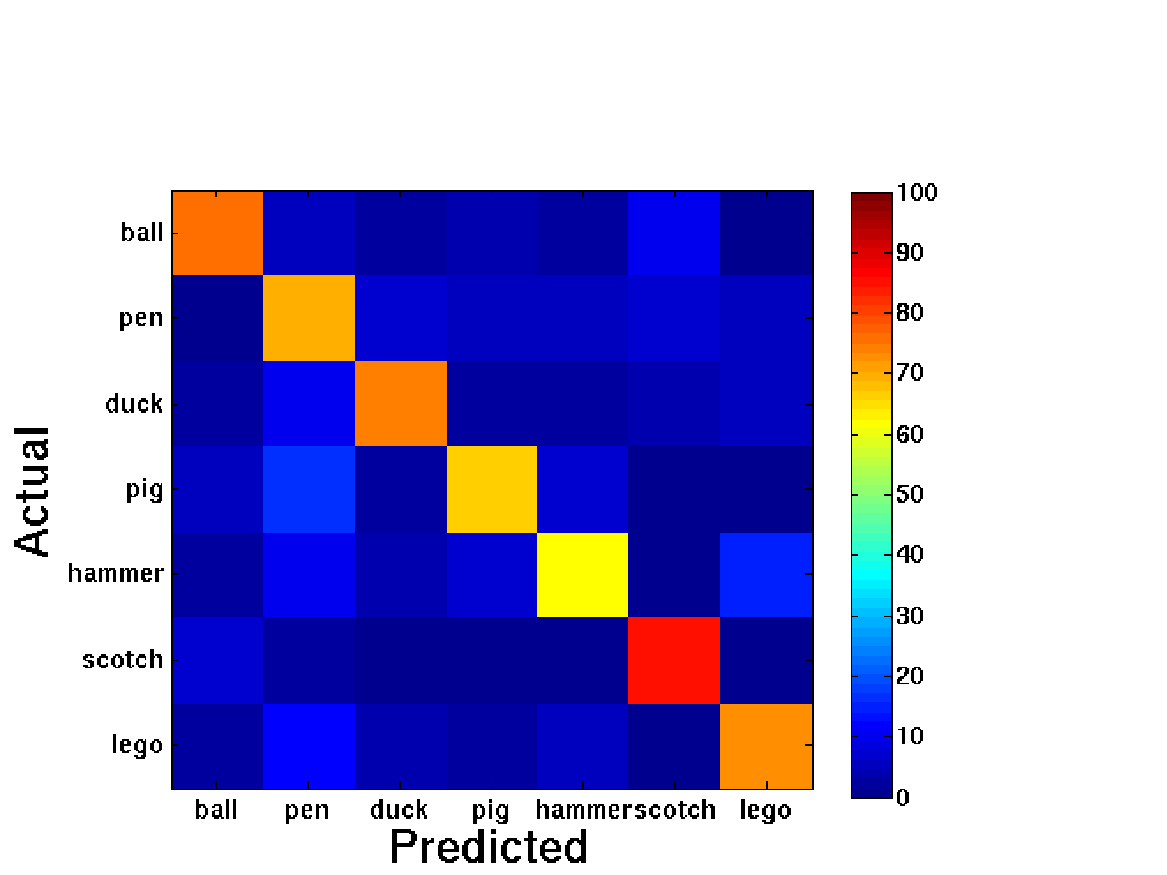
\includegraphics[width=0.25\textwidth]{images/conf_mot_ric.pdf} \\
(a) & (b) & (c)\\
    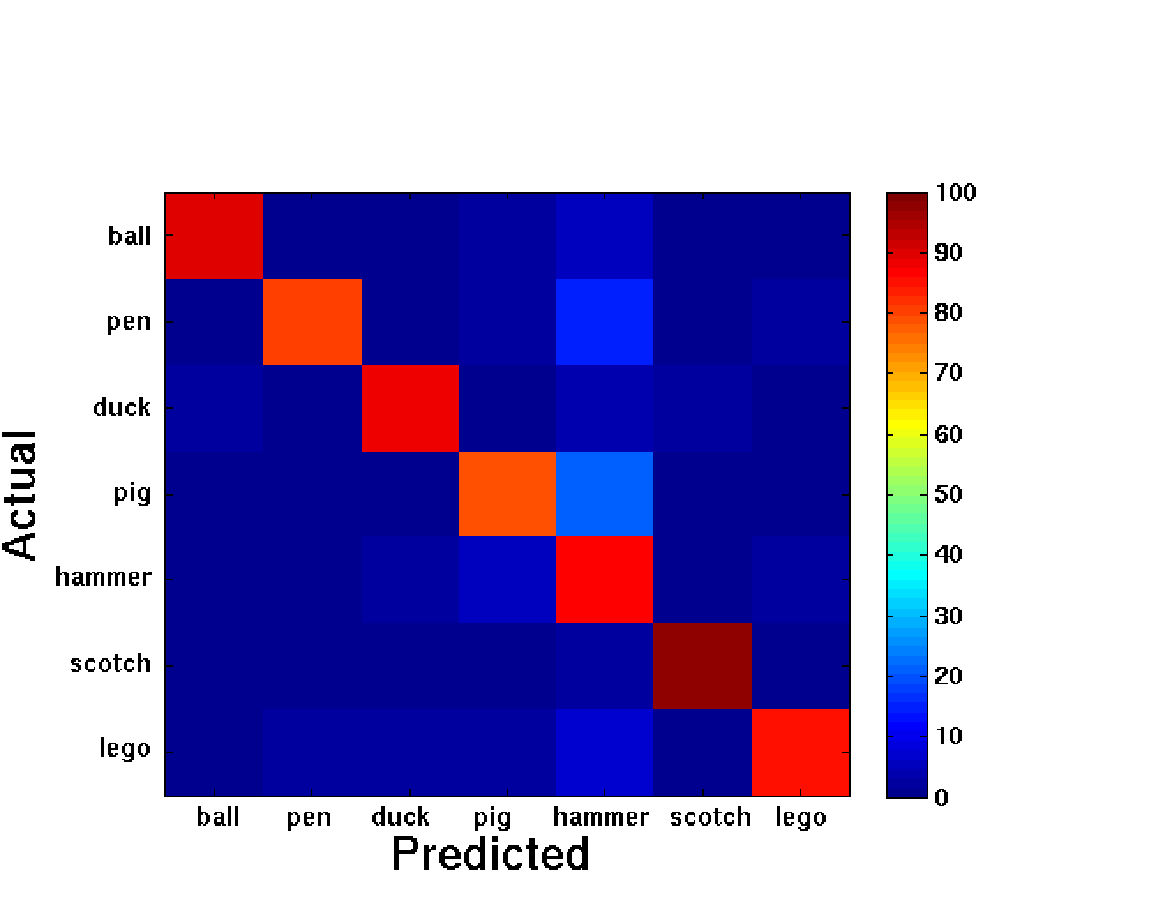
\includegraphics[width=0.25\textwidth]{images/conf_low_ric.pdf} &
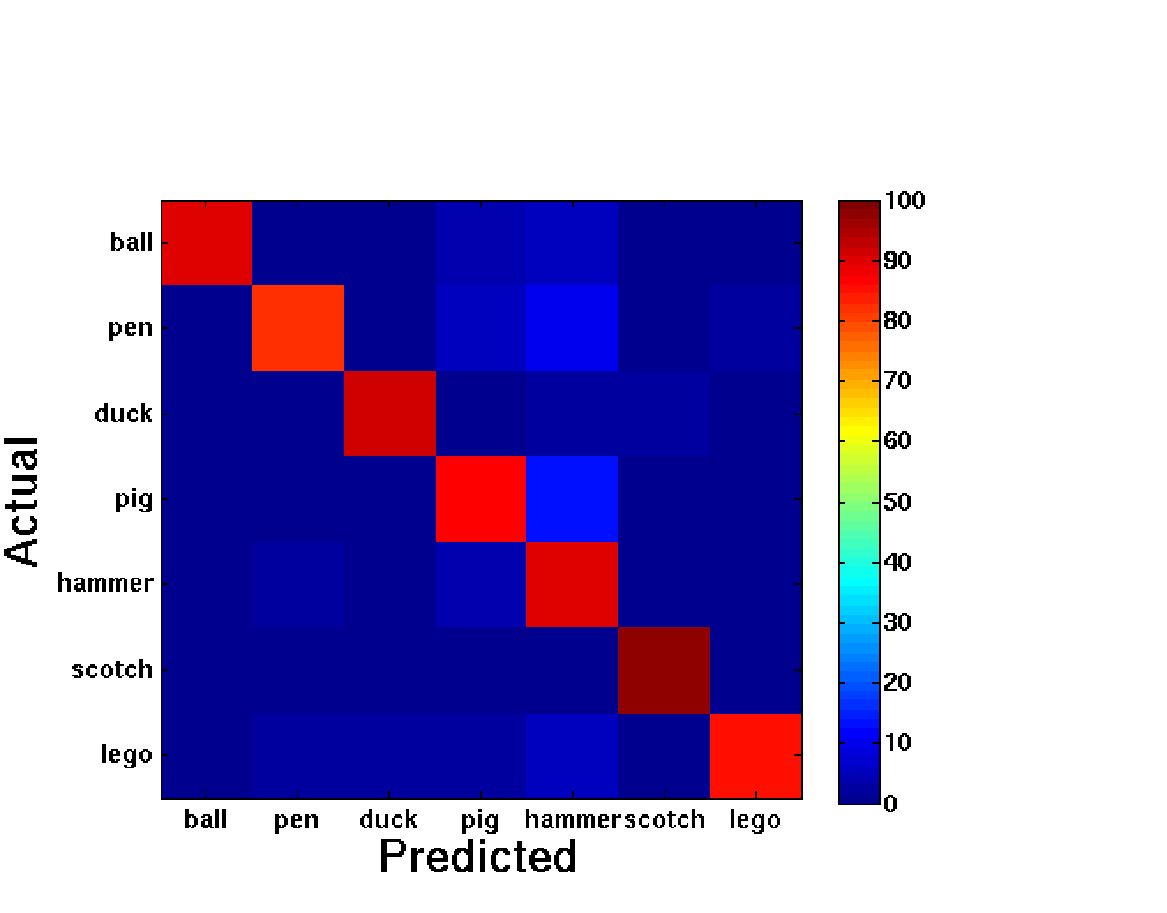
\includegraphics[width=0.25\textwidth]{images/conf_mck_ric.pdf} &
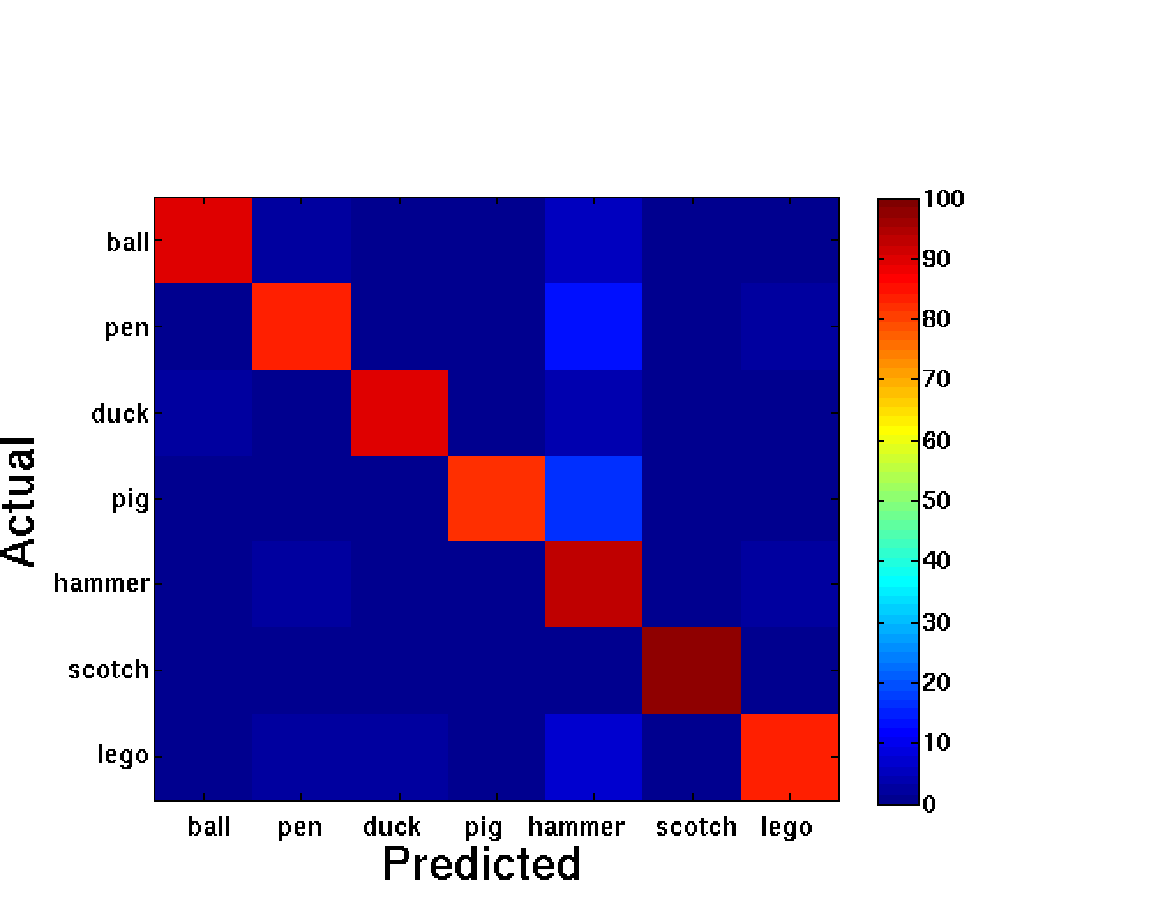
\includegraphics[width=0.25\textwidth]{images/conf_das_ric.pdf} \\
    (d) & (e) & (f)\\
  \end{tabular}
  \caption{(a) Classification mean accuracy of the seven objects averaged
    on the ten splits; (b) confusion matrix using visual features; (c) confusion
    matrix using motor features; (d) confusion matrix using the low-level
    feature integration; (e) confusion matrix using the mid-level
    feature integration; (f) confusion matrix using the high-level
    feature integration.}
  \label{fig:rec_data}
\end{figure*}


Results are reported in Figure \ref{fig:rec_data}. Figure \ref{fig:rec_data}-a shows the recognition rates obtained by using 
only visual information (V -- the same shown in the previous section), only motor information (M), and the two combined together 
(LOW, MID, HIGH). 
We see that using the archetypal grasps as motor information, the performance of the motor only classifier slightly decreases compared to
what we obtained on real motor features: $71.90\%\pm2.06\%$  obtained with the archetypal grasps, as opposed to the
$75.53\%\pm1.22\%$ obtained using real motor features. Still the performance of the multi-modal classifiers show an increase in the overall performance,
compared to the vision only approach.
Once again, the best performance is achieved by MCK (88.77\%$\pm$ 1.29\%), closely followed by DAS (88.38\%$\pm$ 1.31\%).

%Using the motor information we obtain a mean accuracy of $71.90\%\pm2.06\%$, and the mid level integration with the visual features brings to $88.77\%\pm1.29\%$. Overall the combination of the two modalities leads to a statistically significative
%advanatege: the gain in accuracy between MCK and only using visual features is $2.40\%\pm1.05\%$ (difference in accuracy evaluated per split and then averaged on the 10 splits).

Figure \ref{fig:rec_data}-b, -f 
shows the confusion matrices obtained by 
all classifiers, as reported in Section \ref{res:real}.
%the vision only classifier (Figure \ref{fig:rec_data}-b), by the 
%sensorymotor only classifier (Figure \ref{fig:rec_data}-c) and by the MCK classifier (Figure \ref{fig:rec_data}-d). 
We see that the results for the reconstructed motor data are in general lower than that obtained with the
real ones (Figure \ref{fig:real_data}-c). To explain this behaviour there are two things to keep in mind: (1) the lower is the number of
possible grasps associated with an object, the fewer are the data on which the corresponding neural
network is trained; (2) if the first step of hypothesis generation  fails, the error propagates
on the motor data reconstruction. In particular, both points give an intuition about why the objects ``pig'' and ``hammer'' (which were manipulated with only one grasp each) present the worst recognition results using motor
information ($66.65\%$ and $61.45\%$ respectively). Nevertheless, in the ``pig'' case, 
the reconstructed grasp data added to the visual features brings the mean accuracy for object recognition from 
$75.1\%$ (only visual) to $87.0\%$ (using MCK).
As a last remark, we see once again that MCK obtains the best performance (gain in accuracy of $2.40\%$) and therefore it appears to be the most
suitable candidate for the VMC module.





%\subsection{Discussion}
%\label{res:discussion}

%{\bf FIXME BABS: la scrivo quando c'e' un primo draft completo degli esperimenti}

%\begin{itemize}
% \item action dinamic discarded till now
% \item bad visual features, they do not capture the object 3d shape
% \item very simple regression strategy
%\end{itemize}
